\documentclass{article}
% %%%%%%%%%%%%%%%%%%%%%%%%%%%%%%%%%%%%%%%%%
% % LaTeX Template
% % Version 1.0
% %
% % This template originates from:
% % http://www.LaTeXTemplates.com
% %
% % Authors:
% % Rocco Lo Russo (https://github.com/roccolr)
% %%%%%%%%%%%%%%%%%%%%%%%%%%%%%%%%%%%%%%%%%


%----------------------------------------------------------------------------------------
%	PACKAGES AND OTHER DOCUMENT CONFIGURATIONS
%----------------------------------------------------------------------------------------

\usepackage{amsmath,amsfonts,stmaryrd,amssymb} % Math packages

\usepackage[ddmmyyyy]{datetime}
\usepackage{enumerate} % Custom item numbers for enumerations

\usepackage[ruled]{algorithm2e} % Algorithms

\usepackage[framemethod=tikz]{mdframed} % Allows defining custom boxed/framed environments

\usepackage{listings} % File listings, with syntax highlighting
\usepackage[hidelinks]{hyperref}

\lstset{
  language=C,
  basicstyle=\ttfamily\small\color{black},
  numbers=left,
  numberstyle=\small\color{gray},
  stepnumber=1,
  numbersep=4pt,
  frame=single,
  rulecolor=\color{black},
  framesep=5pt,
  xleftmargin=20pt,
  framexleftmargin=15pt,
  breaklines=true,
  showstringspaces=false,
  keywordstyle=\color{purple}\bfseries,          % parole chiave (if, else, int, return...)
  commentstyle=\color{teal}\itshape,           % commenti
  stringstyle=\color{orange},                   % stringhe
  identifierstyle=\color{black},                % identificatori normali
  emph={size_t, uint32_t, uint64_t, TAS, RTE},            % tipi aggiuntivi
  emphstyle=\color{blue}\bfseries,            % stile tipi aggiuntivi
  morekeywords={uint8_t, uint16_t, uint32_t, uint64_t, int8_t, int16_t, int32_t, int64_t, bool, true, false}, % tipi e parole chiave extra
  morecomment=[l]{//},                           % commenti con //
  morecomment=[s]{/*}{*/},                       % commenti multilinea
}

\lstdefinelanguage{RISCAsm}{
  morekeywords={
    ADDQ, SUM, ANDI, MOVE,MOVEA, MOVEM, DC, DS, sra, 
    lw, sw, li, la, mv, 
    BEQ, BNE, JMP, CMP, jalr, ret, 
    NOP, lui, RTE, RTS, 
    ecall, ebreak, ORG, EQU, JSR, CLR, TAS 
  },
  sensitive=true,
  morecomment=[l]{\*},
  morestring=[b]",
  basicstyle=\ttfamily\small\color{black},
  keywordstyle=\color{purple}\bfseries,
  commentstyle=\color{teal}\itshape,
  stringstyle=\color{orange},
  numbers=left,
  numberstyle=\small\color{gray},
  stepnumber=1,
  numbersep=4pt,
  frame=single,
  rulecolor=\color{black},
  framesep=5pt,
  xleftmargin=20pt,
  framexleftmargin=15pt,
  showstringspaces=false,
  breaklines=true,
}

%----------------------------------------------------------------------------------------
%	DOCUMENT MARGINS
%----------------------------------------------------------------------------------------

\usepackage{geometry} % Required for adjusting page dimensions and margins

\geometry{
	paper=a4paper, % Paper size, change to letterpaper for US letter size
	top=2.5cm, % Top margin
	bottom=3cm, % Bottom margin
	left=2.5cm, % Left margin
	right=2.5cm, % Right margin
	headheight=14pt, % Header height
	footskip=1.5cm, % Space from the bottom margin to the baseline of the footer
	headsep=1.2cm, % Space from the top margin to the baseline of the header
	%showframe, % Uncomment to show how the type block is set on the page
}

%----------------------------------------------------------------------------------------
%	FONTS
%----------------------------------------------------------------------------------------

\usepackage[utf8]{inputenc} % Required for inputting international characters
\usepackage[T1]{fontenc} % Output font encoding for international characters

\usepackage{XCharter} % Use the XCharter fonts
\usepackage{enumitem}
\usepackage{xcolor}
\usepackage{tikz} 
\usetikzlibrary{positioning}

% pseudocode environment %


%----------------------------------------------------------------------------------------
%	COMMAND LINE ENVIRONMENT
%----------------------------------------------------------------------------------------

% Usage:
% \begin{commandline}
%	\begin{verbatim}
%		$ ls
%		
%		Applications	Desktop	...
%	\end{verbatim}
% \end{commandline}

\mdfdefinestyle{commandline}{
	leftmargin=10pt,
	rightmargin=10pt,
	innerleftmargin=15pt,
	middlelinecolor=black!50!white,
	middlelinewidth=2pt,
	frametitlerule=false,
	backgroundcolor=black!5!white,
	frametitle={Command Line},
	frametitlefont={\normalfont\sffamily\color{white}\hspace{-1em}},
	frametitlebackgroundcolor=black!50!white,
	nobreak,
}

% Define a custom environment for command-line snapshots
\newenvironment{commandline}{
	\medskip
	\begin{mdframed}[style=commandline]
}{
	\end{mdframed}
	\medskip
}

%----------------------------------------------------------------------------------------
%	FILE CONTENTS ENVIRONMENT
%----------------------------------------------------------------------------------------

% Usage:
% \begin{file}[optional filename, defaults to "File"]
%	File contents, for example, with a listings environment
% \end{file}

\mdfdefinestyle{file}{
    innertopmargin=1.6\baselineskip,
    innerbottommargin=0.8\baselineskip,
    topline=false, bottomline=false,
    leftline=false, rightline=false,
    leftmargin=2cm,
    rightmargin=2cm,
    singleextra={
        \draw[fill=black!10!white](P)++(0,-1.2em)rectangle(P-|O);
        \node[anchor=north west] at(P-|O){\ttfamily\mdfilename};
        \def\l{3em}
        \draw(O-|P)++(-\l,0)--++(\l,\l)--(P)--(P-|O)--(O)--cycle;
        \draw(O-|P)++(-\l,0)--++(0,\l)--++(\l,0);
    },
}

% Comando per tab a 4 spazi all’interno dell’ambiente file
\newenvironment{file}[1][File]{%
    \medskip
    \newcommand{\mdfilename}{#1}
    % Rende il carattere tab attivo e lo definisce come 4 spazi
    \catcode`\^^I=\active
    \def^^I{\hspace*{4ex}}%
    \begin{mdframed}[style=file]
}{%
    \end{mdframed}
    \medskip
}

%----------------------------------------------------------------------------------------
%	NUMBERED QUESTIONS ENVIRONMENT
%----------------------------------------------------------------------------------------

% Usage:
% \begin{question}[optional title]
%	Question contents
% \end{question}

\mdfdefinestyle{question}{
	innertopmargin=1.2\baselineskip,
	innerbottommargin=0.8\baselineskip,
	roundcorner=5pt,
	nobreak,
	singleextra={%
		\draw(P-|O)node[xshift=1em,anchor=west,fill=white,draw,rounded corners=5pt]{%
		Question \theQuestion\questionTitle};
	},
}

\newcounter{Question} % Stores the current question number that gets iterated with each new question

% Define a custom environment for numbered questions
\newenvironment{question}[1][\unskip]{
	\bigskip
	\stepcounter{Question}
	\newcommand{\questionTitle}{~#1}
	\begin{mdframed}[style=question]
}{
	\end{mdframed}
	\medskip
}

%----------------------------------------------------------------------------------------
%	WARNING TEXT ENVIRONMENT
%----------------------------------------------------------------------------------------

% Usage:
% \begin{warn}[optional title, defaults to "Warning:"]
%	Contents
% \end{warn}

\mdfdefinestyle{warning}{
	topline=false, bottomline=false,
	leftline=false, rightline=false,
	nobreak,
	singleextra={%
		\draw(P-|O)++(-0.5em,0)node(tmp1){};
		\draw(P-|O)++(0.5em,0)node(tmp2){};
		\fill[black,rotate around={45:(P-|O)}](tmp1)rectangle(tmp2);
		\node at(P-|O){\color{white}\scriptsize\bf !};
		\draw[very thick](P-|O)++(0,-1em)--(O);%--(O-|P);
	}
}

% Define a custom environment for warning text
\newenvironment{warn}[1][Warning:]{ % Set the default warning to "Warning:"
	\medskip
	\begin{mdframed}[style=warning]
		\noindent{\textbf{#1}}
}{
	\end{mdframed}
}

%----------------------------------------------------------------------------------------
%	INFORMATION ENVIRONMENT
%----------------------------------------------------------------------------------------

% Usage:
% \begin{info}[optional title, defaults to "Info:"]
% 	contents
% 	\end{info}

\mdfdefinestyle{info}{%
	topline=false, bottomline=false,
	leftline=false, rightline=false,
	nobreak,
	singleextra={%
		\fill[black](P-|O)circle[radius=0.4em];
		\node at(P-|O){\color{white}\scriptsize\bf i};
		\draw[very thick](P-|O)++(0,-0.8em)--(O);%--(O-|P);
	}
}

% Define a custom environment for information
\newenvironment{info}[1][Info:]{ % Set the default title to "Info:"
	\medskip
	\begin{mdframed}[style=info]
		\noindent{\textbf{#1}}
}{
	\end{mdframed}
}
 % Include the file specifying the document structure and custom commands

% ----------------------------------------------------------------------------------------
% TITOLO
% ----------------------------------------------------------------------------------------
\title{Generic Title}
\author{Mario Giordano \\ \texttt{mario.giordano@pietropacciani.it}}
\date{Università di Firenze --- \today}

% ----------------------------------------------------------------------------------------
\begin{document}


\maketitle

\section*{Introduzione}
Lorem ipsum dolor sit amet consectetur adipiscing elit. Quisque faucibus ex sapien vitae pellentesque sem placerat. 

% TAVOLA DEI CONTENUTI
\tableofcontents
\newpage


\section{Section 1}
\subsection{Subsection 1.1}
Lorem ipsum dolor sit amet consectetur adipiscing elit.

\begin{equation}
Pietro = Pacciani \implies E = mc^2
\end{equation}

\subsection{Subsection 1.2}
\begin{lstlisting}[language=C]
#include <stdio.h>
#include <stdlib.h>

int main(int argc, char ** argv){
    printf("Ritorneremo prima o dopo!\n");
    return 0;
}
\end{lstlisting}

\begin{commandline}
\begin{verbatim}
$ gcc pacciani.c -o pacciani.exe
$ ./pacciani.exe se nimmondo... 
eistesse un po di bene
\end{verbatim}
\end{commandline}

\begin{center}
\begin{minipage}{0.5\linewidth}
\begin{algorithm}[H]
\KwIn{$A$, array di n pietro pacciani}
A.heap\_size = 1 \;
\For{$i=2$ to A.lenght}{
    MAX\_HEAP\_INSERT(A, A[i])
}
\caption{\texttt{build\_max\_heap\_v2}}
\end{algorithm}
\end{minipage}
\end{center}

\begin{equation}
I = \int_{a}^{b} f(x) \; \text{d}x.
\end{equation}

\begin{info}
Questo è un blocchetto informativo di esempio.
\end{info}

\begin{question}
Quisque ullamcorper placerat ipsum.
\begin{enumerate}[label=\alph*)]
\item Do this.
\item Do that.
\item Do something else.
\end{enumerate}
\end{question}

\begin{center}
\begin{minipage}{0.5\linewidth}
\begin{algorithm}[H]
\KwIn{$(a, b)$, due numeri floating-point}
\KwResult{$(c, d)$, tali che $a+b = c+d$}
\If{$|b| > |a|$}{
  scambia $a$ e $b$\;
}
$c \leftarrow a+b$\;
$z \leftarrow c-a$\;
$d \leftarrow b-z$\;
\Return $(c,d)$\;
\caption{\texttt{FastTwoSum}}
\end{algorithm}
\end{minipage}
\end{center}

\begin{question}[\itshape (with optional title)]
Mappa della memoria:

\end{question}
\begin{center}
    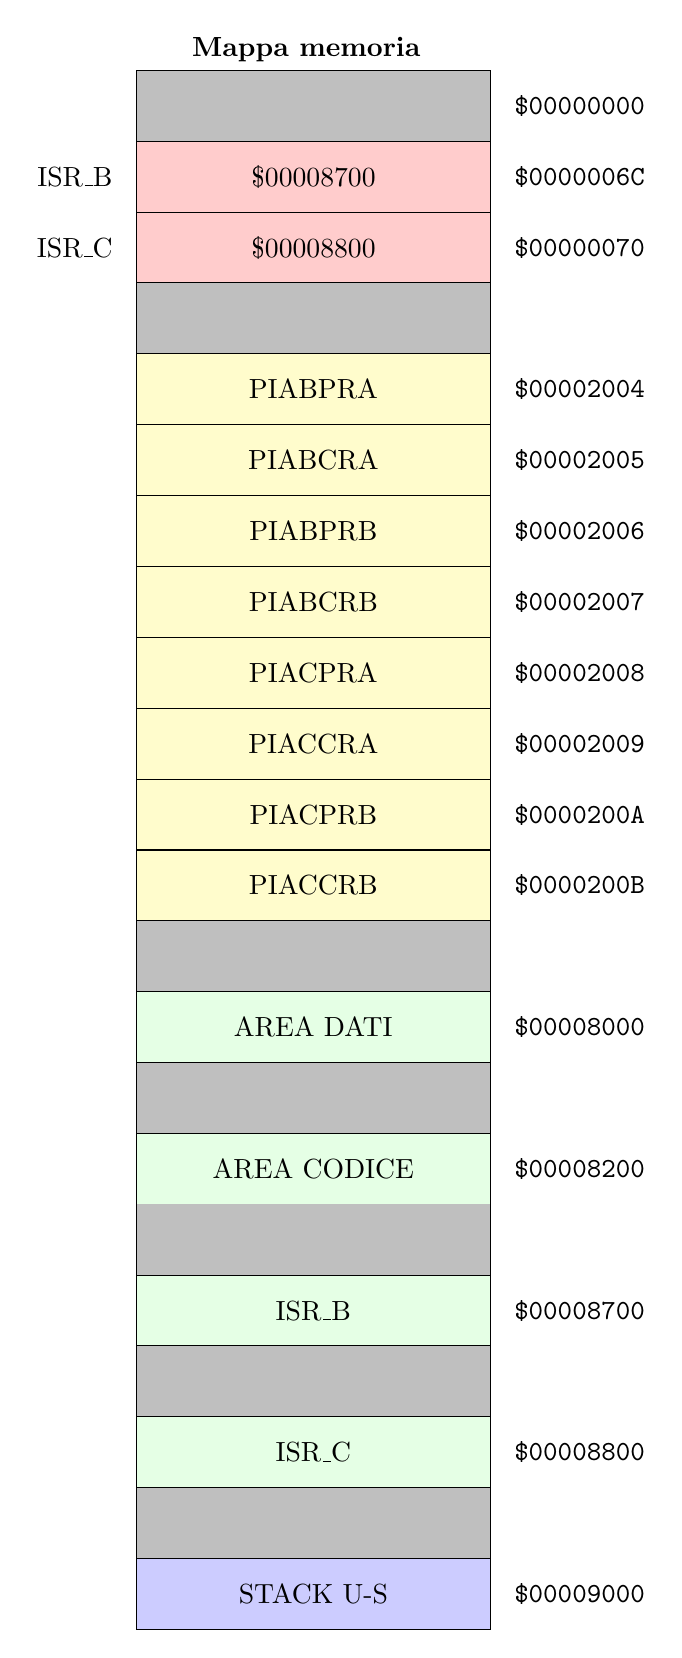
\begin{tikzpicture}[scale=0.9]
        % Rettangolo principale
        \draw (0,0) rectangle (5,20);
        \node at (2.4,20.3) {\textbf{Mappa memoria}};
        
        % vuoto
        \draw (0,20) rectangle (5,19);
        \node[right=5pt] at (5,19.5) {\texttt{\$00000000}};
        \fill[lightgray] (0,20) rectangle (5,19);
        % INT3
        \fill[red!20](0,19) rectangle (5,17);
        \draw (0,19) rectangle (5,18);
        \node[left=5pt] at (0,18.5) {ISR\_B};
        \node[right=5pt] at (5,18.5) {\texttt{\$0000006C}};
        \node at (2.5,18.5) {\$00008700}; 
        
        % INT4 
        \draw (0,18) rectangle (5,17);
        \node[left=5pt] at (0,17.5) {ISR\_C};
        \node[right=5pt] at (5,17.5) {\texttt{\$00000070}};
        \node at (2.5,17.5) {\$00008800};

        % vuoto
        \draw (0,17) rectangle (5,16);
        \fill[lightgray] (0,17) rectangle (5,16);
        %PIA 
        \fill[yellow!20](0,16) rectangle (5,8);
        \draw(0,16) rectangle (5,15);
        \node[right=5pt] at (5,15.5) {\texttt{\$00002004}};
        \node at (2.5,15.5) {PIABPRA};
        \draw(0,15) rectangle (5,14);
        \node[right=5pt] at (5,14.5) {\texttt{\$00002005}};
        \node at (2.5,14.5) {PIABCRA};
        \draw(0,14) rectangle (5,13);
        \node[right=5pt] at (5,13.5) {\texttt{\$00002006}};
        \node at (2.5,13.5) {PIABPRB};
        \draw(0,13) rectangle (5,12);
        \node[right=5pt] at (5,12.5) {\texttt{\$00002007}};
        \node at (2.5,12.5) {PIABCRB};

        \draw(0,12) rectangle (5,11);
        \node[right=5pt] at (5,11.5) {\texttt{\$00002008}};
        \node at (2.5,11.5) {PIACPRA};
        \draw(0,11) rectangle (5,10);
        \node[right=5pt] at (5,10.5) {\texttt{\$00002009}};
        \node at (2.5,10.5) {PIACCRA};
        \draw(0,10) rectangle (5,9);
        \node[right=5pt] at (5,9.5) {\texttt{\$0000200A}};
        \node at (2.5,9.5) {PIACPRB};
        \draw(0,9) rectangle (5,8);
        \node[right=5pt] at (5,8.5) {\texttt{\$0000200B}};
        \node at (2.5,8.5) {PIACCRB};

        % vuoto
        \draw (0,8) rectangle (5,7);
        \fill[lightgray] (0,8) rectangle (5,7);
        
        % DATI
        \fill[green!10] (0,7) rectangle (5,0);
        \draw(0,7) rectangle (5,6);
        \node[right=5pt] at (5,6.5) {\texttt{\$00008000}};
        \node at (2.5,6.5) {AREA DATI};

        
        % vuoto
        \draw (0,6) rectangle (5,5);
        \fill[lightgray] (0,6) rectangle (5,5);
        
        % CODICE
        \draw(0,5) rectangle (5,4);
        \node[right=5pt] at (5,4.5) {\texttt{\$00008200}};
        \node at (2.5,4.5) {AREA CODICE};

        % vuoto
        \draw (0,4) rectangle (5,3);
        \fill[lightgray] (0,4) rectangle (5,3);

        % ISRB 
        \draw(0,3) rectangle (5,2);
        \node[right=5pt] at (5,2.5) {\texttt{\$00008700}};
        \node at (2.5,2.5) {ISR\_B};

        % vuoto
        \draw (0,2) rectangle (5,1);
        \fill[lightgray] (0,2) rectangle (5,1);

        % ISRC
        \draw(0,1) rectangle (5,0);
        \node[right=5pt] at (5,0.5) {\texttt{\$00008800}};
        \node at (2.5,0.5) {ISR\_C};

        % vuoto 
        \draw(0,0) rectangle (5,-1);
        \fill[lightgray](0,0) rectangle (5,-1);
        % STACK
        \fill[blue!20](0,-1) rectangle (5,-2);
        \draw (0,-1) rectangle (5,-2);
        \node[right=5pt] at (5,-1.5) {\texttt{\$00009000}};
        \node at (2.5,-1.5) {STACK U-S};

        \draw(0,-2) rectangle (5,20); % ricalco bordi
    \end{tikzpicture}
\end{center}



% Tabella descrittiva
\begin{description}[style=nextline,leftmargin=3.45cm,labelwidth=2.8cm,labelsep=0.6cm,font=\ttfamily\bfseries]
\item[esempio1] Intero che può assumere i valori 0 o 1.
\item[esempio2] Intero che può assumere i valori 0 o 1.
\end{description}

% \begin{lstlisting}
% c code snippet
% \end{lstlisting}

% \begin{lstlisting}[language={[x86masm]Assembler}]
% asm code snippet
% \end{lstlisting}

\begin{warn}[Osservazione:]
Questo è un messaggio di warning.
\end{warn}

\end{document}